复势

引入复变函数的方法研究平面流动问题,若以速度势$\varphi$为实部,流函数$\psi$为虚部,则组成的复函数$w=\varphi+i\psi$称为复势函数,由
$\varphi,\psi$的定义,Cauchy-Riemann方程得到满足:
\begin{equation}\label{eq:82CREq}
\begin{cases}
\frac{\partial \varphi}{\partial x}=& \frac{\partial \psi}{\partial y} \,\,(=u)\\
\frac{\partial \varphi}{\partial y}=& -\frac{\partial \psi}{\partial x}\,\, (=v)
\end{cases}
\end{equation}
所以$w(z)$是解析函数,$\varphi$和$\psi$为一对共轭调和函数。

一般地,由$(x,y)$到$(z,z^*)$的线性变换关系
\begin{equation}
\begin{cases}
x=&\frac{z+z^*}{2}\\
y=&\frac{z-z^*}{2i}
\end{cases}
\end{equation}

可知$\varphi(x,y)+i\psi(x,y)=w(z,z^*)$,可以从下面的推导说明\eqref{eq:82CREq}式是$\frac{\partial w}{\partial z^*}=0$的充要条件,即$w$只与$z$有关。
\begin{align*}
\frac{\partial w}{\partial z^*} = & \frac{\partial w}{\partial x}\frac{\partial x}{\partial z^*}
+\frac{\partial w}{\partial y}\frac{\partial y}{\partial z^*}\\
= & \frac{1}{2}(\frac{\partial \varphi}{\partial x}+i\frac{\partial \psi}{\partial x})
-\frac{1}{2i}\frac{\partial \varphi}{\partial y}+i\frac{\partial \psi}{\partial y}\\
= & \frac{1}{2}(\frac{\partial \varphi}{\partial x}-\frac{\partial \psi}{\partial y})
+\frac{i}{2}(\frac{\partial \psi}{\partial x}+\frac{\partial \varphi}{\partial y})
\end{align*}

对于复势$w(z)$,其导数与求导方向无关,即$\frac{\partial w}{\partial x}=\frac{\partial w}{\partial (iy)}=\frac{dw}{dz}$,
由\eqref{eq:82CREq}式容易得到复速度的表达式:
\begin{equation}\label{eq:82ComplexVelocity}
V=u+iv=\left(\frac{dw}{dz}\right)^*
\end{equation}
平面绕流问题的提法:
\begin{figure}[!ht]
 \centering
 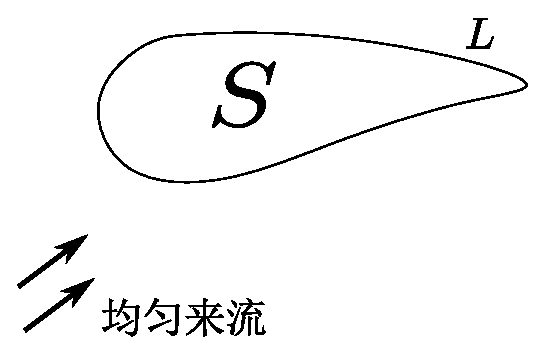
\includegraphics[width=5cm]{streamingProblem.eps}
 \caption{平面绕流问题图示}\label{fig:82StP}
\end{figure}

考虑无穷远的均匀来流通过一截面$S$的流动规律(如图\ref{fig:82StP}),注意到求解域在平面内是双连域,即绕$S$的流线是不可边缘地缩成一个点。一般情况下这类问题
流函数和势函数不具有唯一性,假设有环量条件$\Gamma=\oint_{L} \v{v}\cdot d\v{x}$,则$\varphi=\varphi_p+n\Gamma$均是速度势,其中$n$表示绕$S$转了n圈。

虽然势函数和流函数具有多值性,但速度场是唯一的。事实上,对于双连域中的无旋流场,可以说明任意不可缩周线上的速度环量相等。

\begin{figure}[!ht]
 \centering
 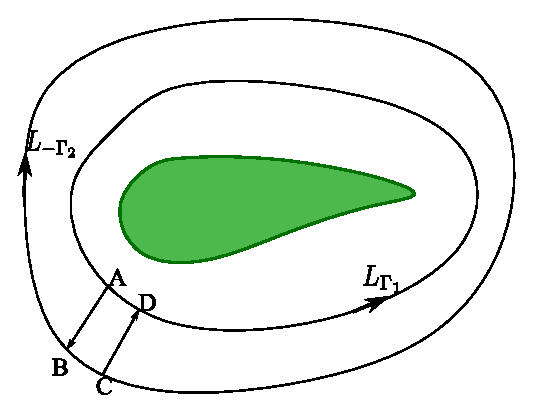
\includegraphics[width=5cm]{doubleConnectedEqualCircuit.eps}
 \caption{速度环量相等推导图示}\label{fig:82doubleConnectedEqualCircuit}
\end{figure}

如图\ref{fig:82doubleConnectedEqualCircuit}所示,对于任取的两条周线$L_{\Gamma_1},L_{\Gamma_2}$,
我们取一个很小的隔面ABCD,其中AD,BC无限靠近,考虑周线,$\v{AB},L_{-\Gamma_2},\v{CD},L_{\Gamma_1}$,该周线可以连续地缩为一个点,因此
其上的速度环量积分为0,又因为AD,BC无限靠近,有$\int_{AB+CD}\v{v}\cdot d\v{x}=0$,所以有
\begin{equation}
\oint_{L_{\Gamma_1}} \v{v}\cdot d\v{x} = \oint_{L_{\Gamma_2}} \v{v}\cdot d\v{x}
\end{equation}


因此$\Gamma$对给定的流场是常数,不会出现在$\nabla \varphi$中。

求解平面绕流问题,如果我们取复势$w(z)$作为未知函数,由于$w(z)$的实部和虚部分别满足Laplace 方程,因此只需要寻找$w(z)$满足一定的
边界条件,即适合以下三类约束:
\begin{itemize}
\item 无穷远处:$\frac{dw}{dz}_{|z\to \infty}=u_{\infty}-iv_{\infty}$
\item 物面上: Im$(w(z))|_L=\psi_{|L}=0$
\item 任意不可缩周线$L$: Re$(\oint_{L} \frac{dw}{dz} dz)=\Gamma$
\end{itemize}

根据流函数的性质,我们可以得到$\frac{dw}{dz}$的环量积分虚部是流量,即有:
\begin{equation}\label{eq:82GQ}
\oint_{L} \frac{dw}{dz} dz = \Gamma + i Q
\end{equation}

用复势求解平面无旋流动问题对于简单的情形可采用奇点叠加法,为此给出下面几类基本解的形式:

\begin{table}[!ht]
\centering
\begin{tabular}{cccccc}
\Xhline{1pt}
&$w(z)$ &等$\varphi$线 & 等$\psi$线 & 周线环量 & 周线流量\\
\hline\noalign{\smallskip}
均匀流 & $(u_{\infty}-iv_{\infty})z$ & $u_{\infty}x+v_{\infty}y=c$ & $u_{\infty}y-v_{\infty}x=c'$ & 0 & 0 \\[0.1cm]
\hline\noalign{\smallskip}
点源(汇) & $\frac{Q}{2\pi} \ln(z-z_0)$ & $|z-z_0|=c$ & arg$(z-z_0)=c'$ & 0 & Q \\[0.1cm]
\hline\noalign{\smallskip}
点涡 & $\frac{\Gamma}{2\pi i} \ln(z-z_0)$ & arg$(z-z_0)=c$ & $|z-z_0|=c'$ & $\Gamma$ & 0 \\[0.1cm]
\hline\noalign{\smallskip}
\multirow{2}{*}{平面偶极子} & \multirow{2}{*}{$\frac{-M}{2\pi} \frac{1}{z-z_0}$} & 过$z_0$,圆心在直线 & 过$z_0$,圆心在直线 & \multirow{2}{*}{0} & \multirow{2}{*}{0} \\
& & $t:z_0+tM$上的圆簇 & $t:z_0+tMi$上的圆簇 & & \\[0.1cm]
\Xhline{1pt}
\end{tabular}
\caption{四类基本解基本性质}\label{tb:82FourBasic}
\end{table}

对于每一类基本解,再给出$w(z)$后,令其实部等于$c$得等$\varphi$线,虚部等于$c'$得等$\psi$线,利用\eqref{eq:82GQ}式
可得周线环量和周线流量。

这里比较特殊的是平面偶极子的复势$w$,仍采用定义$m=\displaystyle\lim_{\delta l \to 0}(Q\delta l)$,这里$m$是正实数,
假设$z_0$处有点汇$-Q$,$z_0'$处有一点源$Q$,定义偶极距为$M=z_0'-z_0=me^{i\beta}$,
利用叠加原理:
\begin{align*}
w(z)=&\lim\limits_{\substack{\delta l\to 0\\Q\delta l \to m}} \left[ \frac{Q}{2\pi}\ln(z-z_0') - \frac{Q}{2\pi}\ln(z-z_0) \right]\\
=& \frac{-m e^{i\beta}}{2\pi}\frac{1}{z-z_0}\\
=& \frac{-M}{2\pi} \frac{1}{z-z_0}
\end{align*}
我们简记$\sigma=|z-z_0|$,$\alpha'=$arg$(z-z_0)$, 则$w(z)=\frac{m}{2\pi\sigma}e^{\pi+\beta-\alpha'}$,
令Re$w(z)$为常数得到$\sigma=c\cos(\beta-\alpha')$,在平面极坐标系下,由图\ref{fig:82circleInPlanarCoordinate}可知该方程表示一个过$z_0$的圆,
圆心在过$z_0$,方向与$M$相同的直线上($c$可以为负数)。对于平面偶极子诱导的复速度,由\eqref{eq:82GQ}式和留数定理可知
\begin{equation}
\Gamma_l + i Q_l = \oint_l \frac{M}{2\pi}\frac{1}{(z-z_0)^2}=0
\end{equation}

\begin{figure}[!ht]
 \centering
 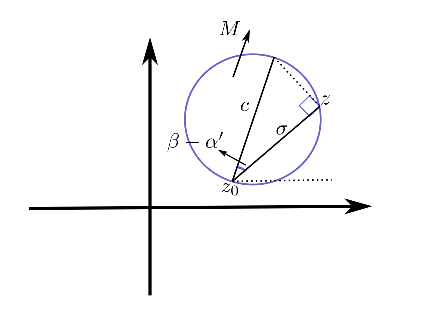
\includegraphics[width=5cm]{circleInPlanarCoordinate.eps}
 \caption{平面极坐标系下圆的方程}\label{fig:82circleInPlanarCoordinate}
\end{figure}

表\ref{tb:82FourBasic}中给出的四类基本解的等$\varphi$线和等$\psi$线的形状在图\ref{fig:82basicSolutionComplexPotential}中表示出来。

\begin{figure}[!ht]
 \centering
 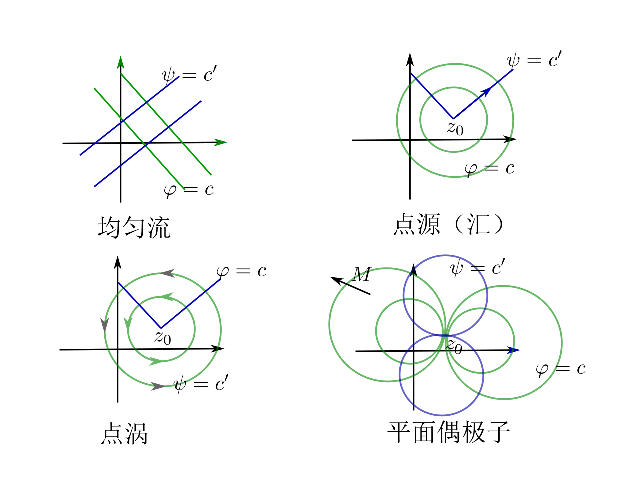
\includegraphics[width=8cm]{basicSolutionComplexPotential.eps}
 \caption{四类基本解等$\varphi$线和等$\psi$线的形状}\label{fig:82basicSolutionComplexPotential}
\end{figure}

基本解的速度场采用公式\eqref{eq:82ComplexVelocity}式可以求出,
\begin{table}[!ht]
\centering
\begin{tabular}{cccccc}
\Xhline{1pt}
&复速度 & 模长 & 幅角\\
\hline\noalign{\smallskip}
均匀流 & $u_{\infty}+i v_{\infty}$ & $|V_{\infty}|$ & $\alpha_{\infty}$\\[0.1cm]
\hline\noalign{\smallskip}
点源(汇) & $\frac{Q}{2\pi \sigma} e^{i\alpha'}$ & $\frac{|Q|}{2\pi \sigma}$ & $\begin{cases}\alpha'&Q>0\\\alpha'+\pi&Q<0\end{cases}$ \\[0.1cm]
\hline\noalign{\smallskip}
点涡 & $\frac{\Gamma}{2\pi \sigma} e^{i(\alpha'+\frac{\pi}{2})}$ & $\frac{|\Gamma|}{2\pi \sigma}$ & $\begin{cases}\alpha'+\frac{\pi}{2}&\Gamma>0\\ \alpha'-\frac{\pi}{2}&\Gamma<0\end{cases}$ \\[0.1cm]
\Xhline{1pt}
\end{tabular}
\caption{基本解的速度场}
\end{table}

%下面简单讨论幂函数$w(z)=Az^n$诱导的速度场,这里$A$是实数,$n>0$。不难写出$v^*=nAz^{n-1}$
% \begin{equation}
% \end{equation}
% \begin{equation}
% \end{equation}
% \begin{equation}
% \end{equation}
% \begin{equation}
% \end{equation}
% \begin{equation}
% \end{equation}
